\documentclass[xcolor=dvipsnames]{beamer}
\usepackage[T1]{fontenc}
\usepackage[utf8]{inputenc}
\usepackage[english,slovak]{babel}

\usepackage{amsmath}
\usepackage{amsthm}
\usetheme{Pittsburgh}
\useoutertheme{shadow}

\usepackage{graphicx}
\usepackage{caption}
\usepackage{subcaption}

\usepackage[]{algorithm2e}
\usepackage{listings}
 \setbeamercovered{transparent}
 \usepackage{cuted}
\usepackage[export]{adjustbox}
\usepackage{mathtools}

\usepackage{lipsum}
\usepackage{verbatim}
\usepackage{transparent}
\usepackage{framed}
\usepackage{xcolor}

\usepackage{multirow}
\usepackage{colortbl}
\usepackage{lmodern}

\newcommand\Wider[2][3em]{%
\makebox[\linewidth][c]{%
  \begin{minipage}{\dimexpr\textwidth+#1\relax}
  \raggedright#2
  \end{minipage}%
  }%
}




\iftrue

\usetheme{Warsaw}

\setbeamercolor{normal text}{fg=white,bg=black!90}
\setbeamercolor{structure}{fg=white}

\setbeamercolor{alerted text}{fg=red!85!black}

\setbeamercolor{item projected}{use=item,fg=black,bg=item.fg!35}

\setbeamercolor*{palette primary}{use=structure,fg=structure.fg}
\setbeamercolor*{palette secondary}{use=structure,fg=structure.fg!95!black}
\setbeamercolor*{palette tertiary}{use=structure,fg=structure.fg!90!black}
\setbeamercolor*{palette quaternary}{use=structure,fg=structure.fg!95!black,bg=black!80}

\setbeamercolor*{framesubtitle}{fg=white}

\setbeamercolor*{block title}{parent=structure,bg=black!60}
\setbeamercolor*{block body}{fg=black,bg=black!10}
\setbeamercolor*{block title alerted}{parent=alerted text,bg=black!15}
\setbeamercolor*{block title example}{parent=example text,bg=black!15}

\fi



%-------------------------------------------------------------------------------------
\title{\color{white} \bf rl}
\author{\color{white} Michal CHOVANEC, PhD}


%\setbeamertemplate{footline}[frame number]{}
\setbeamertemplate{navigation symbols}{}


\date[EURP]{}
\begin{document}

{
    \usebackgroundtemplate
    {
        \vbox to \paperheight{\vfil\hbox to \paperwidth{\hfil

        {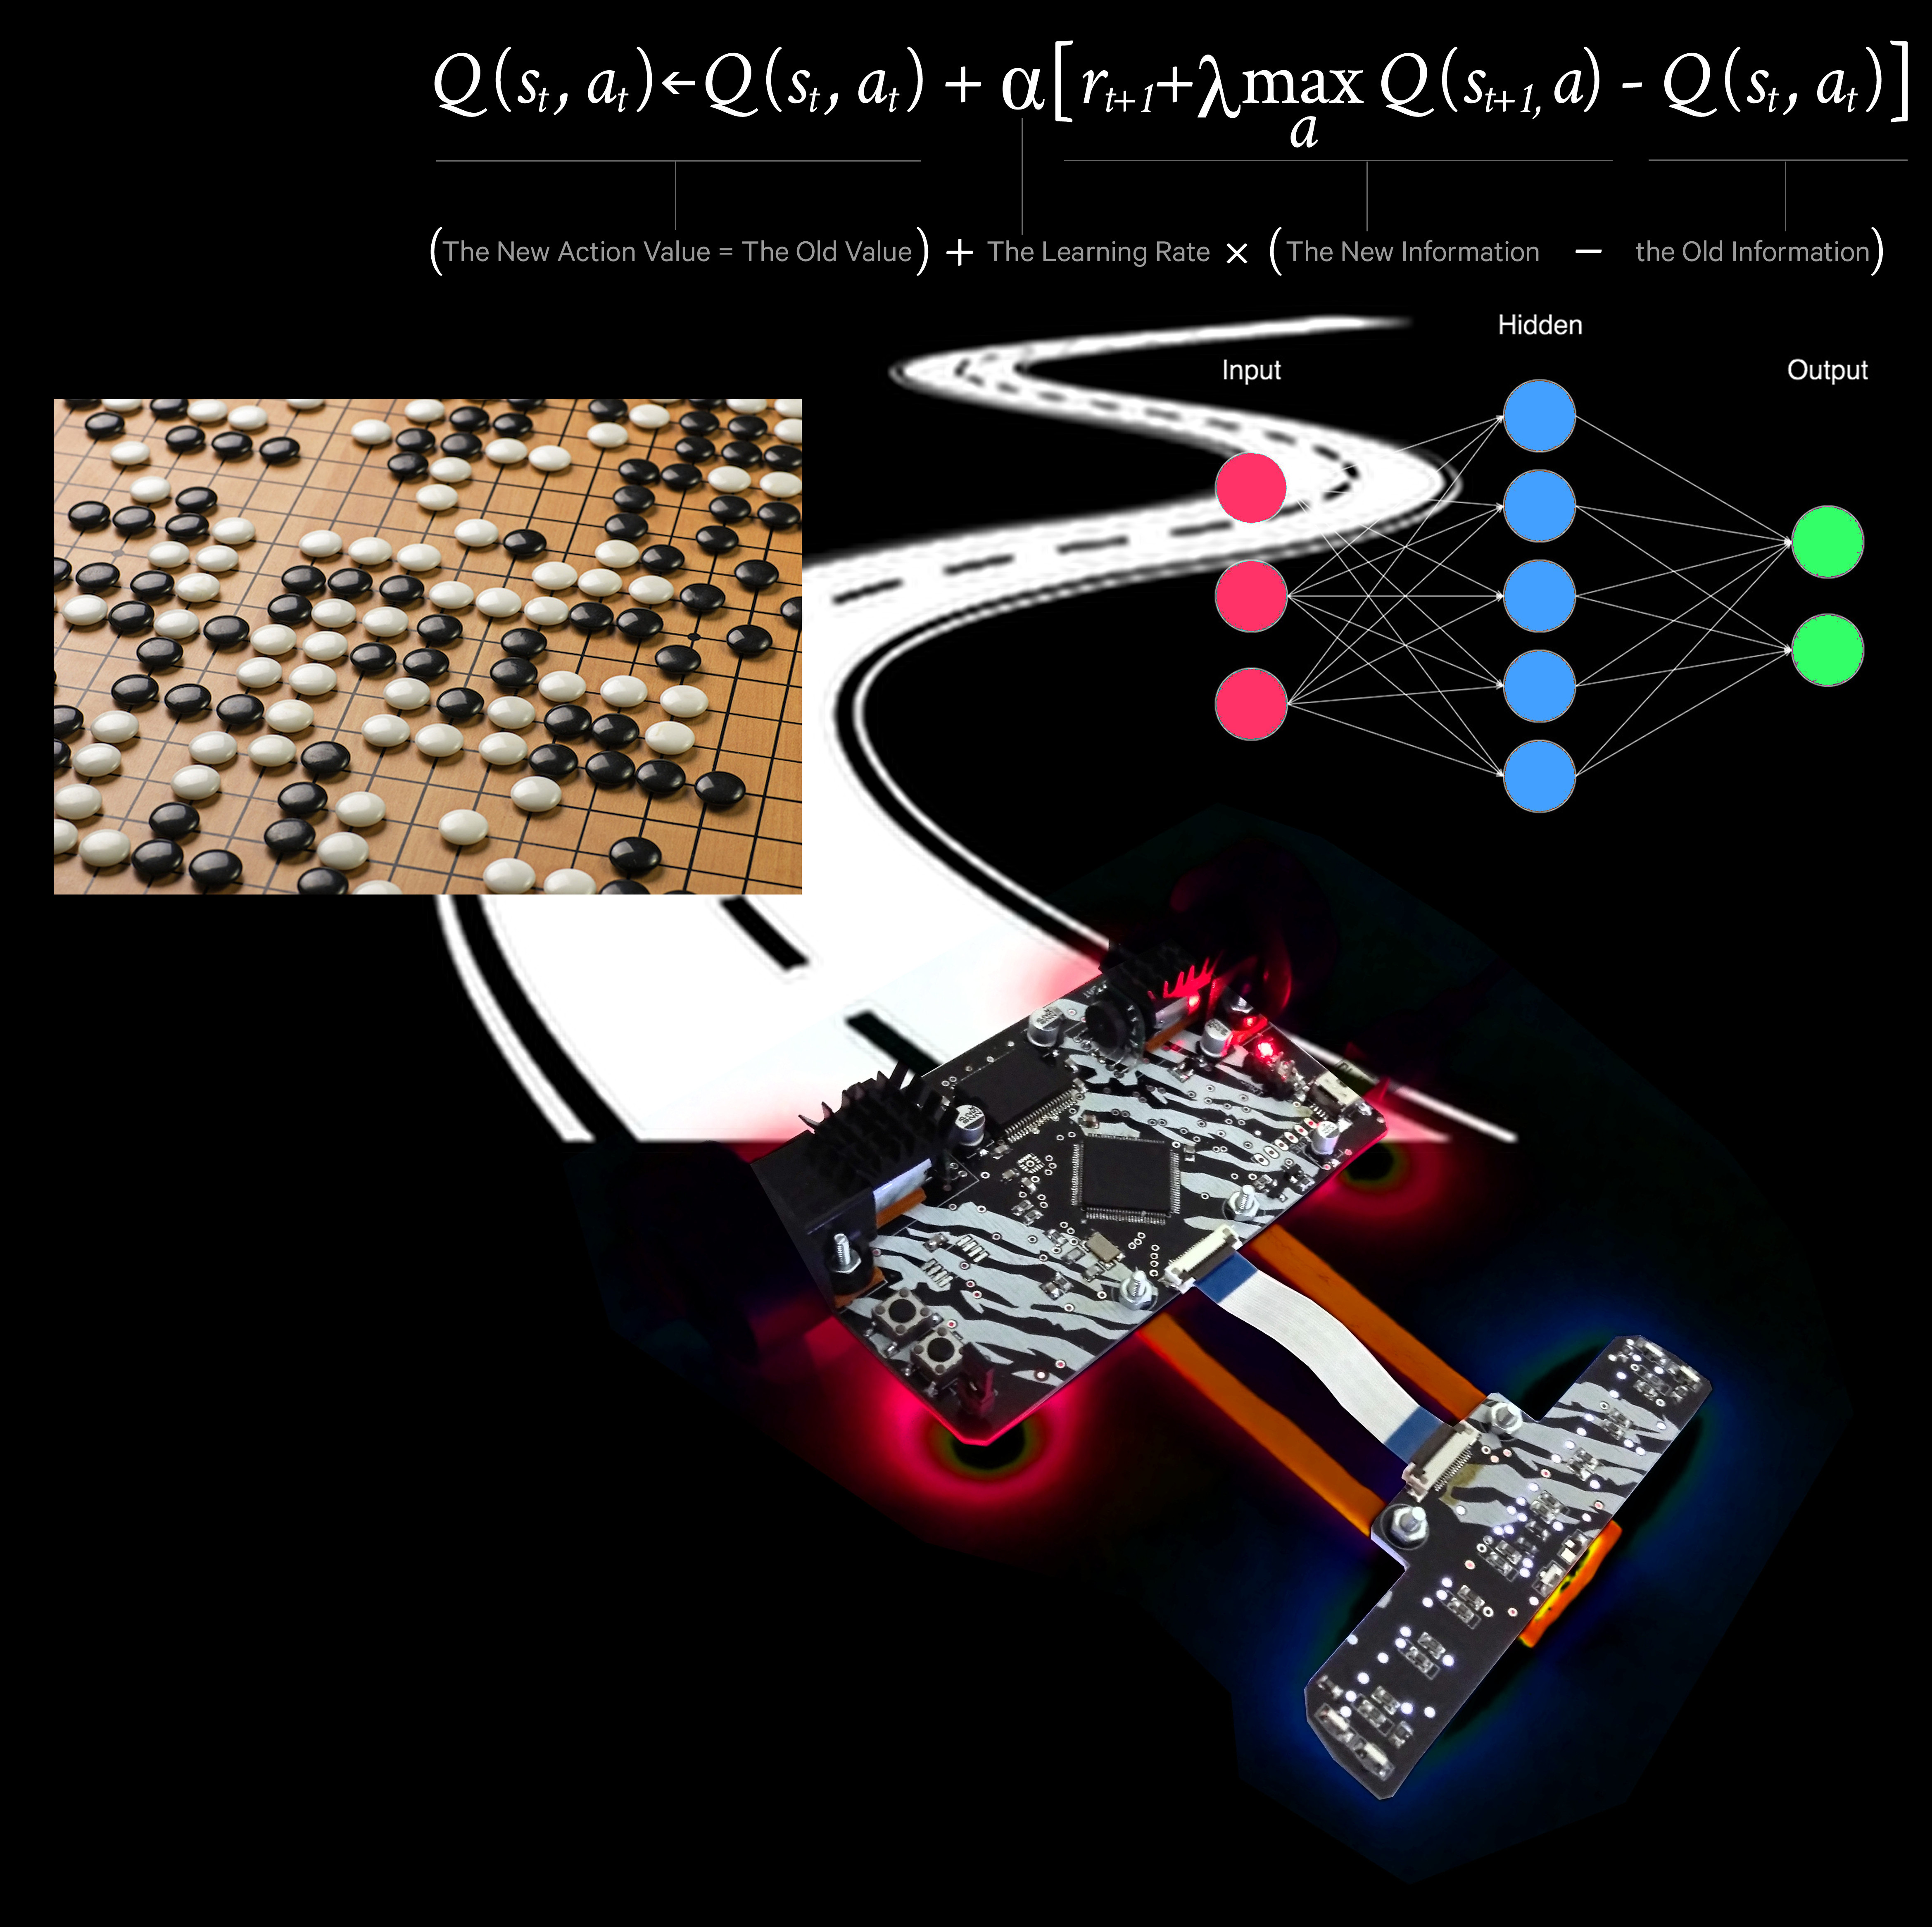
\includegraphics[width=5.05in]{../../pictures/rl_square.jpg}}

        \hfil}\vfil}
    }
    \begin{frame}

    %\titlepage


    \centering
     \colorbox{black}
     {
        \begin{minipage}{7cm}
           {\LARGE \color{white} \bf Deep \\ Reinforcement learning} \\
           {\LARGE \color{white} Michal CHOVANEC, PhD} \\
       \end{minipage}
     }


    \end{frame}
}



\begin{frame}{\bf Atari Bbreakout (arkanoid)}

\begin{columns}
    \begin{column}{0.5\textwidth}

        \begin{figure}
          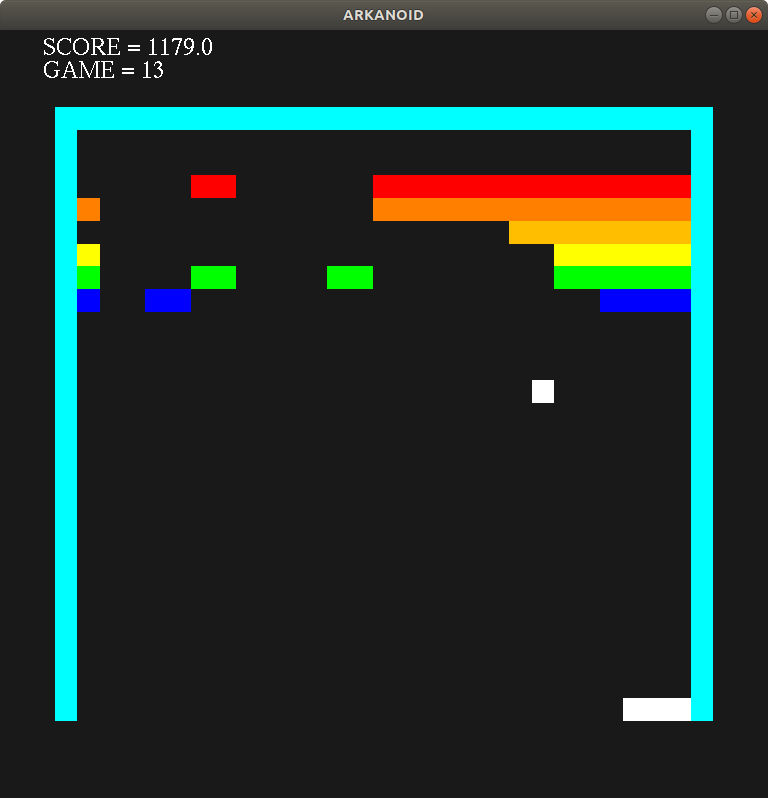
\includegraphics[scale=0.3]{../../pictures/arkanoid.png}
        \end{figure}

    \end{column}
    \begin{column}{0.5\textwidth}

        \begin{itemize}
          \item {\bf state} : screen pixels 16x20x3
          \item {\bf actions} : left, right, no-move
          \item {\bf rewards} :
                \begin{itemize}
                    \item hit $+0.5$
                    \item out $-1.0$
                    \item win $+1.0$
                \end{itemize}
          \item {\bf learn from experiences}, $Q(s, a)$
        \end{itemize}

    \end{column}
\end{columns}

\end{frame}

\begin{frame}{\bf Reinforcement learning}
- learning from punishments and rewards

\begin{itemize}
  \item obtain {\bf state}
  \item choose {\bf action}
  \item {\bf execute} action
  \item obtain {\bf reward}
  \item learn from {\bf experiences}, $Q(s, a)$
\end{itemize}

  \begin{figure}
    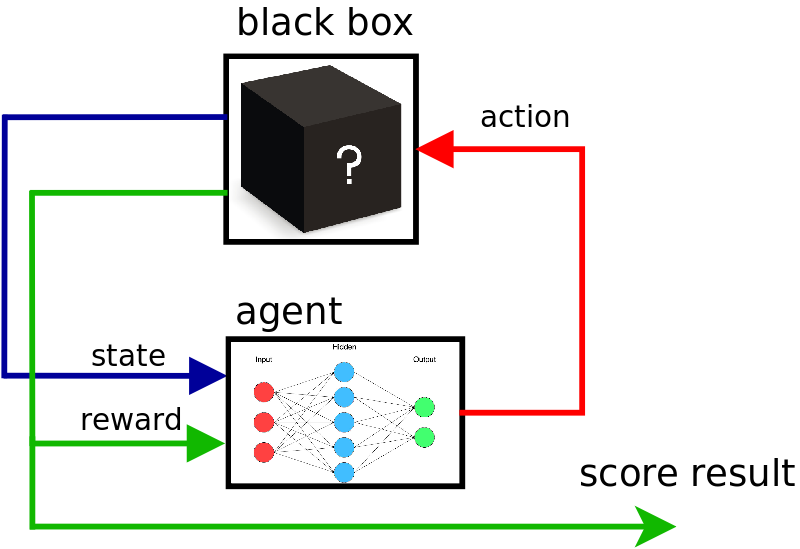
\includegraphics[scale=0.3]{../../diagrams/rl_mechanism.png}
  \end{figure}

\end{frame}


\begin{frame}{\bf What is $Q(s, a)$}

\begin{itemize}
    \item $Q(s, a)$ value of action $a$, executed in state $s$
    \item Q-learning algorithm
        \begin{align*}
        Q'(s, a) = R(s, a) + \gamma \max \limits_{a'} Q(s', a')
        \end{align*}
\end{itemize}

for real problems numbers of states is {\bf too high}
\begin{itemize}
    \item chess $10^{120}$, go $10^{180}$, starcraft $10^{500}$
    \item atoms in observable universe $10^{80}$
    \item neural networks - {\bf deep Q network}
\end{itemize}


\begin{figure}
  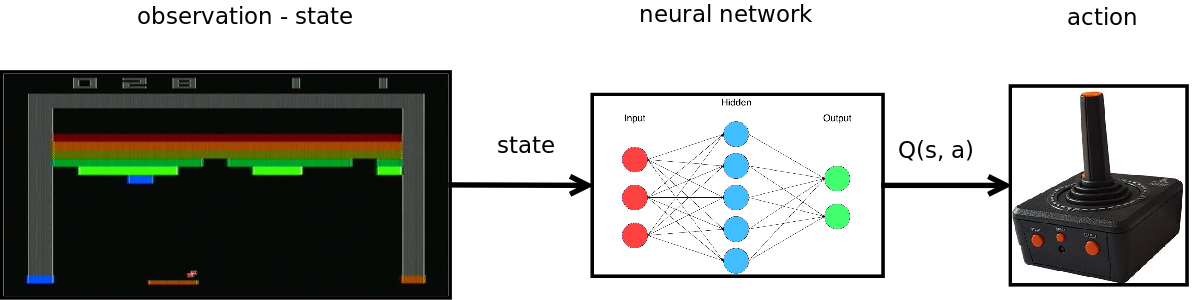
\includegraphics[scale=0.1]{../../diagrams/q_net.png}
\end{figure}


\end{frame}

\begin{frame}{\bf deep Q network - GO playing network example}

{\fontsize{8}{4}\selectfont
total {\bf 412 121 216} computing operations \\
approx. {\bf 8 000 000} parameters to learn
}

\begin{columns}
    \begin{column}{0.2\textwidth}

        \centering
        \begin{figure}
          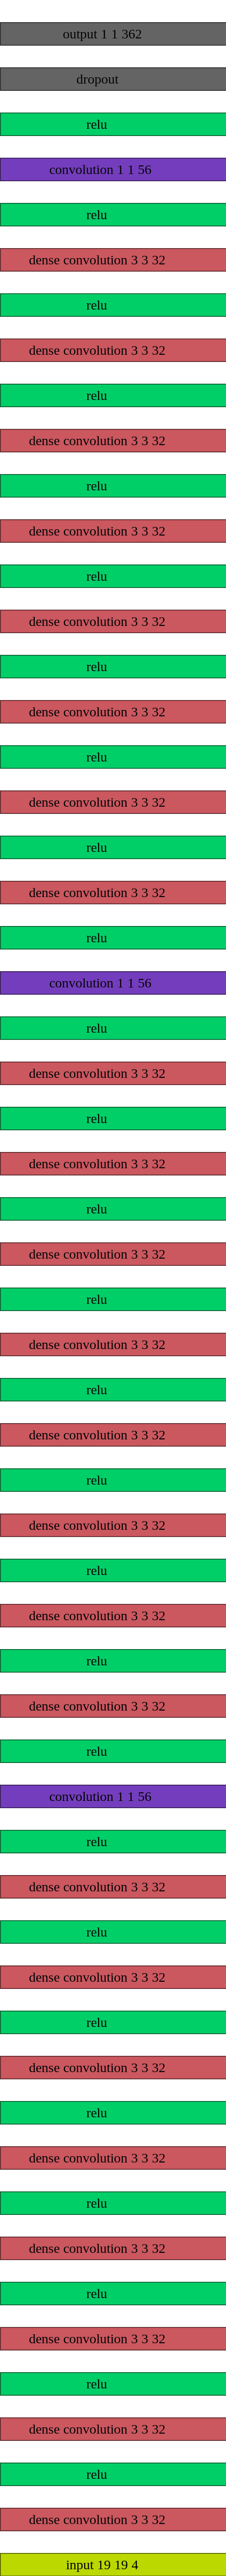
\includegraphics[scale=0.032]{../../pictures/go_cnn_vert.png}
        \end{figure}

    \end{column}
    \begin{column}{0.8\textwidth}

    {\fontsize{8}{3}\selectfont

    \begin{table}[]
    \begin{tabular}{|c|l|l|}
    \hline
    \textbf{layer} & \multicolumn{1}{c|}{\textbf{net 3}}       & \multicolumn{1}{c|}{\textbf{net 5}}       \\ \hline
    0              & \cellcolor[HTML]{FD6864}dense conv 5x5x32 & \cellcolor[HTML]{FD6864}dense conv 3x3x32 \\ \hline
    1              & \cellcolor[HTML]{FD6864}dense conv 5x5x32 & \cellcolor[HTML]{FD6864}dense conv 3x3x32 \\ \hline
    2              & \cellcolor[HTML]{FD6864}dense conv 5x5x32 & \cellcolor[HTML]{FD6864}dense conv 3x3x32 \\ \hline
    3              & \cellcolor[HTML]{FD6864}dense conv 5x5x32 & \cellcolor[HTML]{FD6864}dense conv 3x3x32 \\ \hline
    4              & \cellcolor[HTML]{38FFF8}conv 1x1x32       & \cellcolor[HTML]{FD6864}dense conv 3x3x32 \\ \hline
    5              & \cellcolor[HTML]{FD6864}dense conv 5x5x32 & \cellcolor[HTML]{FD6864}dense conv 3x3x32 \\ \hline
    6              & \cellcolor[HTML]{FD6864}dense conv 5x5x32 & \cellcolor[HTML]{FD6864}dense conv 3x3x32 \\ \hline
    7              & \cellcolor[HTML]{FD6864}dense conv 5x5x32 & \cellcolor[HTML]{FD6864}dense conv 3x3x32 \\ \hline
    8              & \cellcolor[HTML]{FD6864}dense conv 5x5x32 & \cellcolor[HTML]{38FFF8}conv 1x1x56       \\ \hline
    9              & \cellcolor[HTML]{38FFF8}conv 1x1x32       & \cellcolor[HTML]{FD6864}dense conv 3x3x32 \\ \hline
    10             & \cellcolor[HTML]{FD6864}dense conv 5x5x32 & \cellcolor[HTML]{FD6864}dense conv 3x3x32 \\ \hline
    11             & \cellcolor[HTML]{FD6864}dense conv 5x5x32 & \cellcolor[HTML]{FD6864}dense conv 3x3x32 \\ \hline
    12             & \cellcolor[HTML]{FD6864}dense conv 5x5x32 & \cellcolor[HTML]{FD6864}dense conv 3x3x32 \\ \hline
    13             & \cellcolor[HTML]{FD6864}dense conv 5x5x32 & \cellcolor[HTML]{FD6864}dense conv 3x3x32 \\ \hline
    14             & \cellcolor[HTML]{38FFF8}conv 1x1x32       & \cellcolor[HTML]{FD6864}dense conv 3x3x32 \\ \hline
    15             & \cellcolor[HTML]{FD6864}dense conv 5x5x32 & \cellcolor[HTML]{FD6864}dense conv 3x3x32 \\ \hline
    16             & \cellcolor[HTML]{FD6864}dense conv 5x5x32 & \cellcolor[HTML]{FD6864}dense conv 3x3x32 \\ \hline
    17             & \cellcolor[HTML]{FD6864}dense conv 5x5x32 & \cellcolor[HTML]{38FFF8}conv 1x1x56       \\ \hline
    18             & \cellcolor[HTML]{FD6864}dense conv 5x5x32 & \cellcolor[HTML]{FD6864}dense conv 3x3x32 \\ \hline
    19             & \cellcolor[HTML]{38FFF8}conv 5x5x64       & \cellcolor[HTML]{FD6864}dense conv 3x3x32 \\ \hline
    20             & \cellcolor[HTML]{67FD9A}fc 362            & \cellcolor[HTML]{FD6864}dense conv 3x3x32 \\ \hline
    21             &                                           & \cellcolor[HTML]{FD6864}dense conv 3x3x32 \\ \hline
    22             &                                           & \cellcolor[HTML]{FD6864}dense conv 3x3x32 \\ \hline
    23             &                                           & \cellcolor[HTML]{FD6864}dense conv 3x3x32 \\ \hline
    24             &                                           & \cellcolor[HTML]{FD6864}dense conv 3x3x32 \\ \hline
    25             &                                           & \cellcolor[HTML]{FD6864}dense conv 3x3x32 \\ \hline
    26             &                                           & \cellcolor[HTML]{38FFF8}conv 1x1x64       \\ \hline
    27             &                                           & \cellcolor[HTML]{67FD9A}fc 362            \\ \hline
    \end{tabular}
    \end{table}
    }

    \end{column}
\end{columns}


\end{frame}


\begin{frame}{\bf Playing GO (October 2017)}


  \begin{columns}
  \begin{column}{0.5\textwidth}

    \begin{figure}[!htb]
      \centering
      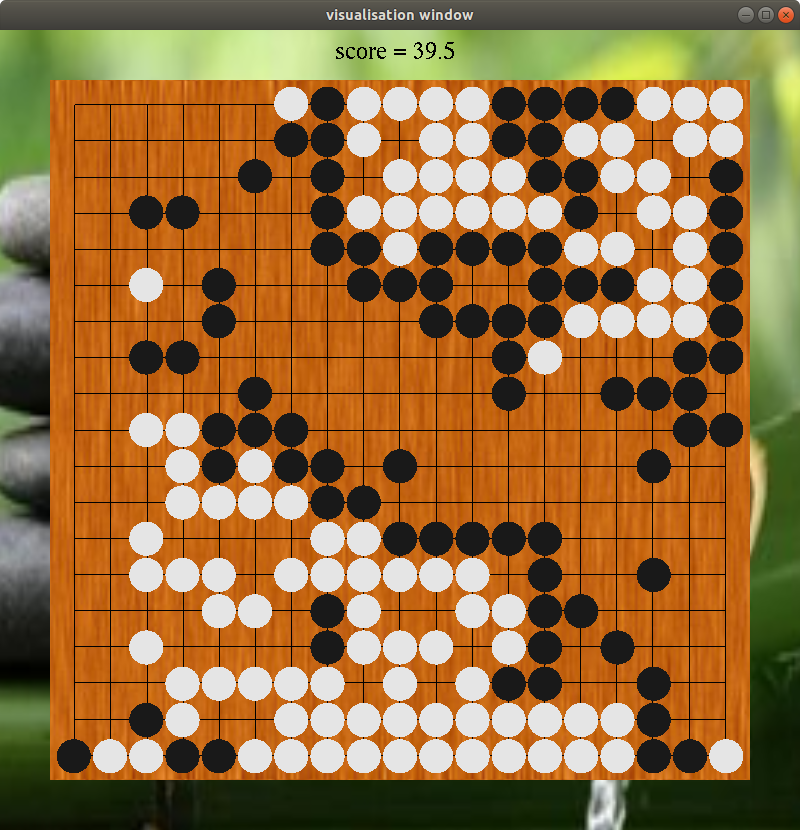
\includegraphics[scale=0.18]{../../pictures/go_board.png}
    \end{figure}


  \end{column}
  \begin{column}{0.5\textwidth}  %%<--- here

    \scriptsize
    {
      \begin{itemize}
        \item {\bf supervised training} - train game using Masters games
        \item {\bf reinforcement learning} - let play two networks against each other
      \end{itemize}
    }
  \end{column}
  \end{columns}

\end{frame}




\begin{frame}{\bf Q\&A}

\begin{figure}
  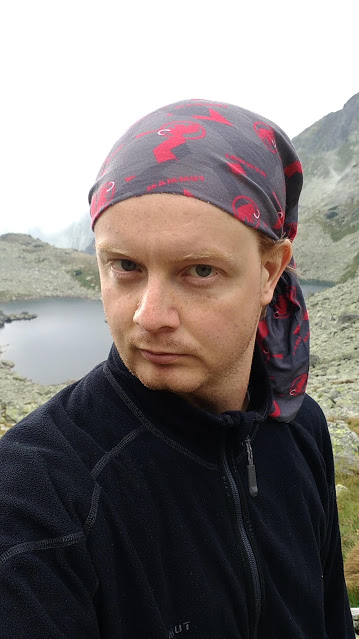
\includegraphics[scale=0.25]{../../pictures/me.jpg}
\end{figure}

\centering {
michal chovanec (michal.nand@gmail.com)
\url{www.youtube.com/channel/UCzVvP2ou8v3afNiVrPAHQGg}
}

\centering {
github
\url{https://github.com/michalnand}
}

\end{frame}


\end{document}
